\subsubsection{\textit{Players service}}
\label{sec:players-service}

El \textit{players service} es el encargado de gestionar la información de los jugadores y su acceso a los mundos.
El servicio se divide en dos componentes principales: la gestión de la información del personaje y el mecanismo
de acceso a los mundos mediante tokens.
\vspace{0.25cm}

Cada jugador dispone de un perfil asociado a su cuenta, cuya información puede actualizarse mediante
\texttt{PATCH /player/character}. La petición debe incluir el nombre del personaje, de forma opcional su biografía y 
la configuración de \textit{skin} (cosmeticos elegidos). El nombre del perfil debe ser único en el sistema; si 
ya está en uso, se retorna un error de conflicto.
\vspace{0.25cm}

Internamente, la actualización se realiza en tres pasos: primero se actualiza la información base del personaje,
luego se eliminan los \textit{sprites} de las categorías marcadas para borrado y finalmente se insertan o
actualizan los nuevos \textit{sprites} por categoría. La consulta de la información de un personaje se realiza
mediante \texttt{GET /player/character} para el usuario autenticado, o mediante \texttt{GET /player/character/\{id\}} 
para consultar el personaje de otro jugador.
\vspace{0.25cm}

\begin{figure}[H]
    \centering
    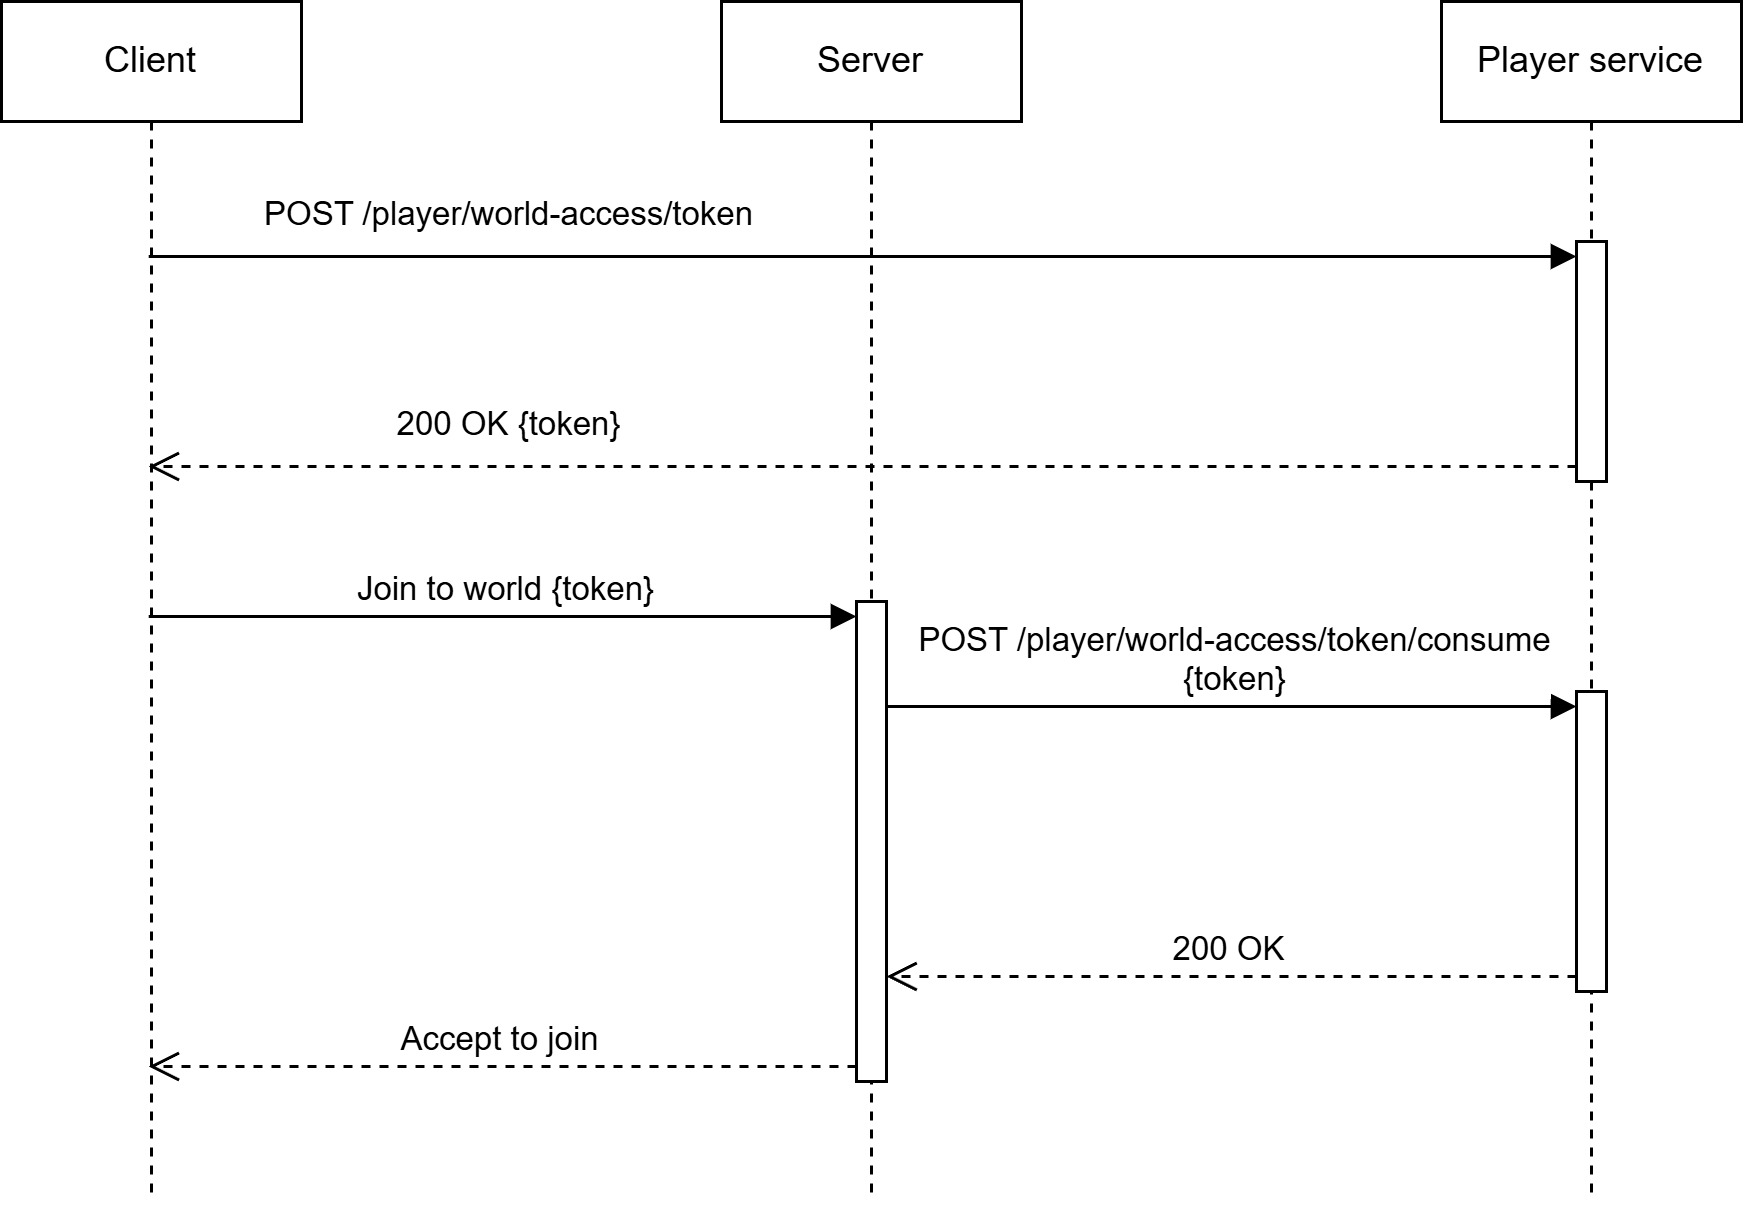
\includegraphics[width=0.85\textwidth]{img/09-technical-details/core-service/players-service-case-1.jpg}
    \caption{Diagrama de secuencia del consumo de un token para unirse a un mundo}
    \label{fig:players-service-case-1}
\end{figure}

Para que un jugador pueda unirse a un mundo, el sistema emplea un mecanismo de tokens de un solo uso. Cuando
un jugador desea unirse a un mundo, solicita un token mediante \texttt{POST /player/world-access/token},
indicando el \texttt{world\_id} de destino. El sistema verifica que el usuario disponga de un personaje creado,
condición necesaria para poder unirse a cualquier mundo; de no tenerlo, retorna un error. Si la validación es
exitosa, se genera un token con una validez de 5 minutos y se persiste en la base de datos.
\vspace{0.25cm}

Una vez emitido, el token es consumido por el servidor del mundo mediante
\texttt{POST /player/} \texttt{world-access/token/consume}, enviando el \texttt{token\_id} recibido. El sistema valida
que el token exista, no haya expirado y no haya sido consumido previamente; cualquiera de estas condiciones
retorna un error específico. Si el token es válido, se marca como consumido y se retorna el identificador del
usuario y del mundo asociados, de modo que el servidor pueda autenticar al jugador que intenta conectarse.
\vspace{0.25cm}
